\section{数据稳定性}
\label{sec:transp-stability}

测量得到的初值、源项和速度场总有误差。这些误差会被放大多少？答案与所用的范数有关，也与误差出现在哪个量上有关。

\paragraph{数据误差的$L^p$估计}
输运方程对$u$是线性的，同一速度场下，两个解的差$e$满足同一方程，其初值和源项分别是初值之差$e_0$与源项之差$g_e$。所以只需估计式~\eqref{eq:transp-flow-solution}给出的$e$。

要点是：逆流映射$\bm{\varphi}_{t,s}$的复合不改变函数的最大值，但会改变$L^{p}$范数，因为积分时要换元。这时$J_{s,t}$进入估计。

\begin{theorem}[数据误差的$L^{p}$估计]
\label{thm:transp-lp}
设$\bm{v}$满足条件（V），存在常数$\kappa\geq0$使$\nabla\cdot\bm{v}\leq\kappa$。设$1\leq p<\infty$，$e_0\in L^{p}(\mathbb{R}^{d})$，$g_e\in L^{1}(0,T;L^{p}(\mathbb{R}^{d}))$，$e$由式~\eqref{eq:transp-flow-solution}给出。则对$t\in[0,T]$，
\begin{equation}
  \lVert e(\cdot,t)\rVert_{p}\leq\mathrm{e}^{\kappa t/p}\lVert e_0\rVert_{p}
  +\int_0^{t}\mathrm{e}^{\kappa(t-s)/p}\lVert g_e(\cdot,s)\rVert_{p}\,\mathrm{d}s.
  \label{eq:transp-lp-estimate}
\end{equation}
当$e_0\in L^{\infty}$，$g_e\in L^{1}(0,T;L^{\infty})$时，把上式中的$\mathrm{e}^{\kappa\cdot/p}$换成$1$，无需假设散度有上界，结论对$p=\infty$成立。
\end{theorem}

\begin{proof}
先看单个函数的复合。设$w\in L^{p}$，换元$\bm{y}=\bm{\varphi}_{t,s}(\bm{x})$，即$\bm{x}=\bm{\varphi}_{s,t}(\bm{y})$，体积元多出因子$J_{s,t}(\bm{y})$，得到
\[
  \int\bigl\lvert w\bigl(\bm{\varphi}_{t,s}(\bm{x})\bigr)\bigr\rvert^{p}\,\mathrm{d}\bm{x}
  =\int\lvert w(\bm{y})\rvert^{p}J_{s,t}(\bm{y})\,\mathrm{d}\bm{y}.
\]

由式~\eqref{eq:transp-liouville-solution}和$\nabla\cdot\bm{v}\leq\kappa$，$J_{s,t}\leq\mathrm{e}^{\kappa(t-s)}$。开$p$次方，
\[
  \lVert w\circ\bm{\varphi}_{t,s}\rVert_{p}\leq\mathrm{e}^{\kappa(t-s)/p}\lVert w\rVert_{p}.
\]

把这个估计用于式~\eqref{eq:transp-flow-solution}的第一项，以及第二项中被积函数的$L^p$范数，再用Minkowski积分不等式把范数移入积分号，就得到式~\eqref{eq:transp-lp-estimate}。对$p=\infty$，复合映射双射，本性上确界不变，同样的步骤给出结论，$J$不再出现。
\end{proof}

式~\eqref{eq:transp-lp-estimate}表明，放大来自局部的体积膨胀：$p$越大，因子$\mathrm{e}^{\kappa t/p}$越接近$1$，$p=\infty$时不放大。

对例~\ref{ex:transp-stretch}的$v=x$，有$\kappa=1$，$J_{0,t}=\mathrm{e}^{t}$是常数。此时$e(x,t)=e_0(x\mathrm{e}^{-t})$，换元得到精确的等式：
\begin{equation}
  \lVert e(\cdot,t)\rVert_{p}=\mathrm{e}^{t/p}\lVert e_0\rVert_{p},
  \label{eq:transp-lp-example}
\end{equation}
所以式~\eqref{eq:transp-lp-estimate}中的因子不能再改进。

密度的情形相反。$\rho$按式~\eqref{eq:transp-density}搬运时，换元给出
\begin{equation}
  \lVert\rho(\cdot,t)\rVert_{p}^{p}=\int\lvert\rho_0(\bm{x})\rvert^{p}\,J_{0,t}(\bm{x})^{1-p}\,\mathrm{d}\bm{x}.
  \label{eq:transp-density-lp}
\end{equation}
$p=1$时$J$的幂次为零，$L^{1}$范数不变，这是质量守恒的范数形式。$p>1$时，密度的误差在压缩处被放大，在膨胀处被缩小，放大倍数由$\inf J_{0,t}$控制。

图~\ref{fig:transp-stability-lp}比较了$v=x$下三角形误差的范数，(a)是$u$的误差，(b)是$\rho$的误差。$u$的$L^{1}$误差增长最快，$L^{\infty}$不变；$\rho$恰好反过来，$L^{1}$不变，$L^{\infty}$衰减最快。线是精确的指数公式，绿点是数值积分。

\begin{BookInlineFigure}
  \centering
  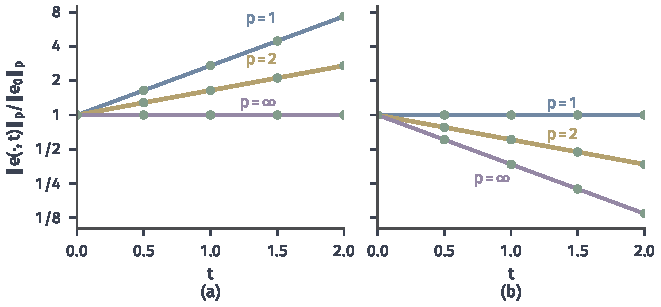
\includegraphics[width=112mm]{figures/06-differential-equations/02-partial-differential-equations/matplotlib/transp-stability-lp/figure.pdf}
  \caption{速度场$v=x$下误差范数的变化（纵轴为对数），$p=1,2,\infty$依次为蓝、黄、紫，绿点是用数值积分算出的范数比。(a)场值误差，满足式~\eqref{eq:transp-lp-example}。(b)密度误差，因子为$\mathrm{e}^{-(1-1/p)t}$。}
  \label{fig:transp-stability-lp}
\end{BookInlineFigure}

\paragraph{比较两个速度场}
现在让速度场本身有误差，初值和源项相同。上面的线性结构用不上了，因为$u^{a}$与$u^{b}$沿不同的轨迹搬运。此时的思路是比较两组特征线，再用数据的空间Lipschitz常数把轨迹差转换为场值差。

\begin{theorem}[速度场误差的$L^{\infty}$估计]
\label{thm:transp-velocity}
设$\bm{v}^{a},\bm{v}^{b}$满足条件（V），其中$\bm{v}^{a}$的常数为$L$，并存在可积函数$\delta$，使
\begin{equation}
  \lVert\bm{v}^{a}(\bm{x},t)-\bm{v}^{b}(\bm{x},t)\rVert_2\leq\delta(t).
  \label{eq:transp-velocity-gap}
\end{equation}
设$u_0$是$L_0$-Lipschitz函数，$f(\cdot,s)$是$L_f$-Lipschitz函数（常数不依赖$s$）。令$u^{a},u^{b}$分别是由式~\eqref{eq:transp-flow-solution}给出的解，定义
\begin{equation}
  E(t,s)=\int_s^{t}\mathrm{e}^{L(r-s)}\delta(r)\,\mathrm{d}r.
  \label{eq:transp-velocity-integral}
\end{equation}
则
\begin{equation}
  \lVert u^{a}(\cdot,t)-u^{b}(\cdot,t)\rVert_{\infty}
  \leq L_0\,E(t,0)+L_f\int_0^{t}E(t,s)\,\mathrm{d}s.
  \label{eq:transp-velocity-estimate}
\end{equation}
\end{theorem}

\begin{proof}
固定$\bm{x}$和$t$，令$\bm{x}^{a}(r)=\bm{\varphi}^{a}_{t,r}(\bm{x})$，$\bm{x}^{b}$同理，$z(r)=\lVert\bm{x}^{a}(r)-\bm{x}^{b}(r)\rVert_2$。两条曲线在$r=t$处重合，从$r$到$t$积分两者的差，
\[
  \bm{x}^{a}(r)-\bm{x}^{b}(r)
  =-\int_r^{t}\bigl(\bm{v}^{a}(\bm{x}^{a},\tau)-\bm{v}^{b}(\bm{x}^{b},\tau)\bigr)\,\mathrm{d}\tau.
\]

在被积函数中加减$\bm{v}^{a}(\bm{x}^{b},\tau)$，第一组差用$L$，第二组差用$\delta$，于是
\[
  z(r)\leq Z(r):=\int_r^{t}\bigl(Lz(\tau)+\delta(\tau)\bigr)\,\mathrm{d}\tau.
\]

由$-Z'(r)=Lz+\delta\leq LZ+\delta$，乘以积分因子，
\[
  \frac{\mathrm{d}}{\mathrm{d}r}\Bigl[\mathrm{e}^{L(r-s)}Z(r)\Bigr]
  =\mathrm{e}^{L(r-s)}\bigl(LZ(r)+Z'(r)\bigr)\geq-\mathrm{e}^{L(r-s)}\delta(r).
\]

从$s$到$t$积分，并用$Z(t)=0$，
\[
  z(s)\leq Z(s)\leq\int_s^{t}\mathrm{e}^{L(r-s)}\delta(r)\,\mathrm{d}r=E(t,s).
\]

这是反向的Gronwall估计，相当于第~\ref{chap:ode-sensitivity}章的结论在时间翻转下的形式。把它代入式~\eqref{eq:transp-flow-solution}，两项分别用$u_0$和$f(\cdot,s)$的Lipschitz常数控制，就得到式~\eqref{eq:transp-velocity-estimate}。
\end{proof}

式~\eqref{eq:transp-velocity-estimate}中$E$的指数因子和$\delta$的时间积分都有明确的含义：时刻$r$的速度误差造成轨迹偏差，沿着剩余的时间由流的拉伸放大，再由数据的斜率转化为场值误差。

取$\bm{v}^{a}=1$，$\bm{v}^{b}=1+\delta$，$f=0$，初值是以$0$为中心、半宽为$1$的三角形。此时$L=0$，$L_0=1$，$E(t,0)=\delta t$，估计给出$\lVert u^{a}-u^{b}\rVert_{\infty}\leq\delta t$。当$\delta t\leq1$时，这恰好是解的实际差：两个三角形错开$\delta t$，在斜边上的差就是$\delta t$。$\delta=0.2$，$t=1.5$时差为$0.3$。

\paragraph{间断初值}
初值有间断时，式~\eqref{eq:transp-velocity-estimate}中的$L_0$是无穷大，估计完全失效。台阶初值$u_0=\mathbf{1}_{x<0}$在$v=1$与$v=1+\delta$下的解，只要$\delta>0$、$t>0$，就总存在宽度为$\delta t$的一段，两解相差$1$，所以
\begin{equation}
  \lVert u^{a}(\cdot,t)-u^{b}(\cdot,t)\rVert_{\infty}=1.
  \label{eq:transp-step-sup}
\end{equation}
一致范数下解对速度场不连续。积分范数则仍然能捕捉到这段宽度的微小：
\begin{equation}
  \lVert u^{a}(\cdot,t)-u^{b}(\cdot,t)\rVert_{p}=(\delta t)^{1/p},\qquad 1\leq p<\infty.
  \label{eq:transp-step-lp}
\end{equation}

图~\ref{fig:transp-velocity-perturb}对比了两种初值。(a)中平滑的三角形错开一点点，差也很小，(b)中台阶错开任意小，最大差都是$1$，但差的区域宽度很窄。(c)把这几个量对$\delta$作图。

\begin{BookInlineFigure}
  \centering
  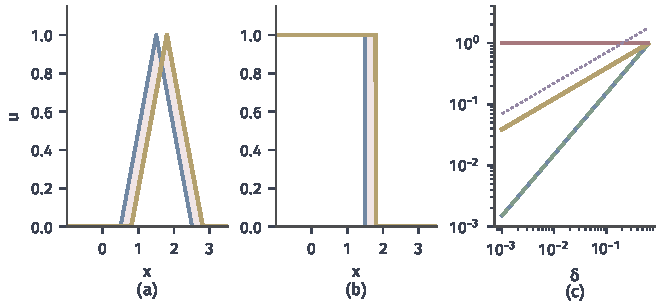
\includegraphics[width=112mm]{figures/06-differential-equations/02-partial-differential-equations/matplotlib/transp-velocity-perturb/figure.pdf}
  \caption{$v=1$（蓝）与$v=1+\delta$（黄）的解，$t=1.5$，$\delta=0.2$，浅红区域是两解的差。(a)三角形初值。(b)台阶初值。(c)误差随$\delta$的变化（对数坐标）：蓝线是三角形的一致误差，与绿色虚线（台阶的$L^{1}$误差）重合，都正比于$\delta$；黄线是台阶的$L^{2}$误差，与紫色点线（参考斜率$1/2$）平行；红线是台阶的一致误差。}
  \label{fig:transp-velocity-perturb}
\end{BookInlineFigure}

式~\eqref{eq:transp-step-lp}的收敛率$1/p$比光滑情形的一阶要慢，$p=2$时只有$1/2$阶。对一般的$L^{p}$初值，收敛仍然成立，只是不再有统一的速率。

\begin{theorem}[粗糙初值的$L^{p}$收敛]
\label{thm:transp-lp-convergence}
设$\bm{v}^{n},\bm{v}$满足条件（V），常数$L$相同，$\nabla\cdot\bm{v}^{n},\nabla\cdot\bm{v}\leq\kappa$，且$\bm{v}^{n}$在$\mathbb{R}^{d}\times[0,T]$上一致收敛于$\bm{v}$。设$u_0\in L^{p}(\mathbb{R}^{d})$，$1\leq p<\infty$，$u^{n},u$是相应的解$u_0\circ\bm{\varphi}^{n}_{t,0}$与$u_0\circ\bm{\varphi}_{t,0}$。则对每个$t\in[0,T]$，
\begin{equation}
  \lVert u^{n}(\cdot,t)-u(\cdot,t)\rVert_{p}\to0.
  \label{eq:transp-lp-convergence}
\end{equation}
\end{theorem}

\begin{proof}
任取$\varepsilon>0$。Lipschitz紧支函数在$L^{p}$中稠密，取这样的$w$，使$\lVert u_0-w\rVert_{p}<\varepsilon$，它的支集在球$B$内，Lipschitz常数为$L_w$。三角不等式给出
\[
  \lVert u^{n}-u\rVert_{p}\leq\lVert(u_0-w)\circ\bm{\varphi}^{n}_{t,0}\rVert_{p}
  +\lVert w\circ\bm{\varphi}^{n}_{t,0}-w\circ\bm{\varphi}_{t,0}\rVert_{p}
  +\lVert(w-u_0)\circ\bm{\varphi}_{t,0}\rVert_{p}.
\]

由定理~\ref{thm:transp-lp}的证明，第一项和第三项都不超过$\mathrm{e}^{\kappa t/p}\varepsilon$。第二项中，定理~\ref{thm:transp-velocity}的第一步给出逐点差不超过$L_wE_n$，其中$E_n\to0$。

被积函数只在$\bm{\varphi}^{n}_{0,t}(B)\cup\bm{\varphi}_{0,t}(B)$上非零，这个集合的体积不超过$2\mathrm{e}^{\kappa t}\lvert B\rvert$，所以第二项不超过
\[
  L_wE_n\bigl(2\mathrm{e}^{\kappa t}\lvert B\rvert\bigr)^{1/p}\to0.
\]
先让$n\to\infty$，再让$\varepsilon\to0$，即得式~\eqref{eq:transp-lp-convergence}。
\end{proof}

定理中$p<\infty$是必需的：式~\eqref{eq:transp-step-sup}就是$p=\infty$的反例。$\varepsilon$的取法依赖$u_0$，所以这里没有速率，这也是间断初值与Lipschitz初值的根本差别。

\paragraph{弱收敛}
数据本身的扰动也可能只在弱意义下小。比如$u_0^{n}(x)=\sin(nx)$在$L^{2}$的有界区间上弱收敛于$0$，但它的$L^{2}$范数不趋于零。

固定速度场，$u_0^{n}\rightharpoonup u_0$（$L^{p}$中弱收敛，$1<p<\infty$）时，对任意$h\in C_c(\mathbb{R}^{d})$，由换元，
\[
  \int u^{n}(\bm{y},t)h(\bm{y})\,\mathrm{d}\bm{y}
  =\int u_0^{n}(\bm{x})\,h\bigl(\bm{\varphi}_{0,t}(\bm{x})\bigr)J_{0,t}(\bm{x})\,\mathrm{d}\bm{x}.
\]

右端的$h(\bm{\varphi}_{0,t}(\cdot))J_{0,t}$是一个固定的$L^{p'}$函数，所以它收敛到对应$u_0$的值。这说明解的弱收敛可以从初值传递过来，但它不提供任何一致的误差估计。上面的振荡初值在$v=x$下的解是$\sin(nx\mathrm{e}^{-t})$，它的振幅始终是$1$，只是积分平均趋于零。
